\chapter{Memory}

\section{RAM access time}
In this part, we report latency for individual integer accesses to main memory and the L1 and L2 caches.

\paragraph{Methodology}
To test memory access latency, I first followed the procedure described in the lmbench paper, testing different stride lengths over varying sizes of arrays. But it is something like sequential access, I wrote code and got the test data, found that it is hard to distinguish different level cache.

Then I choose random access as my methodology. For different array size, I iterate 1 million times, each is random access.

The overhead of random generator and iterations are about  27 cycles.

\paragraph{Predictions}
Different level caches and main memory have different access cycles.

For L1-cache, we predict hardware cycles are 5 and software 2;
For L2-cache, we predict hardware cycles are 10 and software 4;
For L3-cache, we predict hardware cycles are 15 and software 6;
For main memory, we predict hardware cycles are 30 and software 10;

\paragraph{Results}
We present our measure results.

\begin{center}
\begin{tabular}{l*{6}{c}r}
Array size              & Hardware  & Software  & Overall  & Measured  & Remove Overhead \\
\hline
1KB & 5 & 2 & 7 & 28.116605 & 1.116605 \\
2KB & 5 & 2 & 7 & 28.864342 &  1.864342 \\
4KB & 5 & 2 & 7 & 27.687838  & 0.687838\\
8KB & 5 & 2 & 7 & 28.736381  & 1.736381\\
16KB & 5 & 2 & 7 & 28.449469  & 1.449469 \\
32KB & 6 & 3 & 9 & 28.104032  & 1.104032 \\
64KB & 12 & 4 & 16 & 27.939144 &  0.939144\\
128KB & 12 & 4 & 16 & 27.683588 &  0.683588\\
256KB & 14 & 4 & 18 & 28.151352 &  1.151352\\
512KB & 16 & 6 & 22 & 29.170154  & 2.170154 \\
1MB & 16 & 6 & 22 & 32.495250  & 5.495250\\
2MB & 16 & 6 & 22 & 35.461017 & 8.461017 \\
4MB & 20 & 8 & 28 & 47.772894  & 20.772894\\
8MB & 30 & 8 & 38 & 68.281862  & 41.281862\\
16MB & 40 & 10 & 50 & 78.474217 & 51.474217 \\
32MB & 40 & 10 & 50 & 86.430870 & 59.474217 \\
64MB & 40 & 10 & 50 & 84.635278 & 57.635278 \\
\end{tabular}
\end{center}

\begin{figure}[htbp] %  figure placement: here, top, bottom, or page
   \centering
   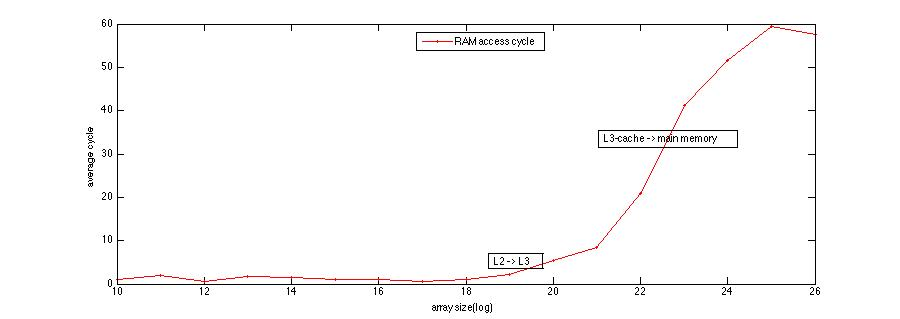
\includegraphics[width=6in]{./pics/ramacc.jpg} 
   \caption{RAM access}
   \label{fig:RAM access}
\end{figure}

\paragraph{Discussion}
It is easy to see the transition from L3-cache to main memory, it is very steep in the picture from array size 22 to 24. Because my L3-cache is 6MB, so it is between 22 and 24.

We can also see the transitions from L2-cache to L3-cache. In the picture, from 18 to 20, the access time increase. Because my L2-cache is 256KB, which is equal to 18 in the picture.

But I can't see the transition from L1-cache to L2-cache in the picture.

We can also see that within cache, the RAM access time cycles are very small compared to that of main memory access.

\section{RAM bandwidth}
In this part, we report bandwidth for both reading and writing.

\paragraph{Methodology}
First, we create an array of size 32 MB that is bigger than L3-cache(6MB) and can be put into memory. In order to reduce the effects of cache line prefetching, we access array as follow : $0 -> HALF\_SIZE -> 1 -> HALF\_SIZE+1 -> ... -> ...$. So we can make sure that each access will cache miss and get from main memory.

To reduce the overhead, we apply loop unrolling. Compared with code that did not apply loop unrolling, the bandwidth increased  a lot.

\paragraph{Predictions}
The machine information tells us that the memory speed is about 1600MB/s. In view of some factors, we predict the speed is 1200 MB/s.

\paragraph{Results}
We present our measure results.

\begin{center}
\begin{tabular}{l*{6}{c}r}
Operation             & Predicted cycle & Measured cycle  \\
\hline
READ & 1200MB/s & 1226MB/s \\
WRITE & 1200MB/s & 1520MB/s \\

\end{tabular}
\end{center}

\paragraph{Discussion}
The actual statistics is very close to our measured results, because we choose well-designed methodology that not only eliminate the effects of cache line prefetching but also use loop unrolling to reduce iteration overhead. That's why we choose 32MB array. Because an array of this size can not be put in cache totally and we can access array to make cache miss.

\section{Page fault service time}
In this part, we report the time for faulting an entire page from disk.

\paragraph{Methodology}
According to the hint, we find that mmap is one useful mechanism. Because file contents are not read from disk initially and do not use physical RAM at all. The actual reads from disk are performed in a "lazy" manner, after a specific location is accessed. Before accessing the content, we record time, after accessing we record again then we can get the page fault service time.

\paragraph{Predictions}
Because my page size is 4 KB, every page fault will loading 4 KB data from disk to memory. SSD read/write speed is fast, so I predict the hardware cycles are 4192 * 2 = 8384 cycles and software cycles are 100.

\paragraph{Results}
We present our measure results.

\begin{center}
\begin{tabular}{l*{6}{c}r}
Operation   & Hardware  & Software  & Overall  & Measured   \\
\hline
Service page fault(cycles) & 8384 & 100 & 8484 & 9898  \\

\end{tabular}
\end{center}

\paragraph{Discussion}
Our estimation is pretty close to the measured result. When a page fault occurs, the program trap into kernel, then kernel load data from disk to memory. 

\paragraph{Question} Dividing by the size of a page, how does it compare to the latency of accessing a byte from main memory?

The page size in our system is 4 KB, so it is approximately 2 cycles per byte of data transfered, compared to about 50 cycles per byte from main memory. May be this is the power of SSD.
